\newpage
\chapter{Umsetzung}

\section{Multicopter Hardware}

Um unsere Plattform testen zu können, haben wir zwei identische Quadcopter aufgebaut.
Wichtig dabei ist, dass für die Benutzung unserer Plattform kein identischer Aufbau nötig ist. Es wird lediglich ein Flight-Controller mit einer MAV-Link kompatiblen Firmware benötigt. z.B. ArduCopter, PX4, usw. 

\subsection{Frame und Antrieb}

Der Frame, die Motoren und ESCs wurden als Kit gekauft. Es handelt sich dabei um ein DJI Flamewheel 450 Frame mit DJI 2312 960kV Motoren und ESeries 420 20A ESCs. Dieses Kit ist weltweit gut verfügbar und deshalb ideal geeignet um einen Versuchsaufbau zu erstellen.

\begin{figure}[h]
	\centering
	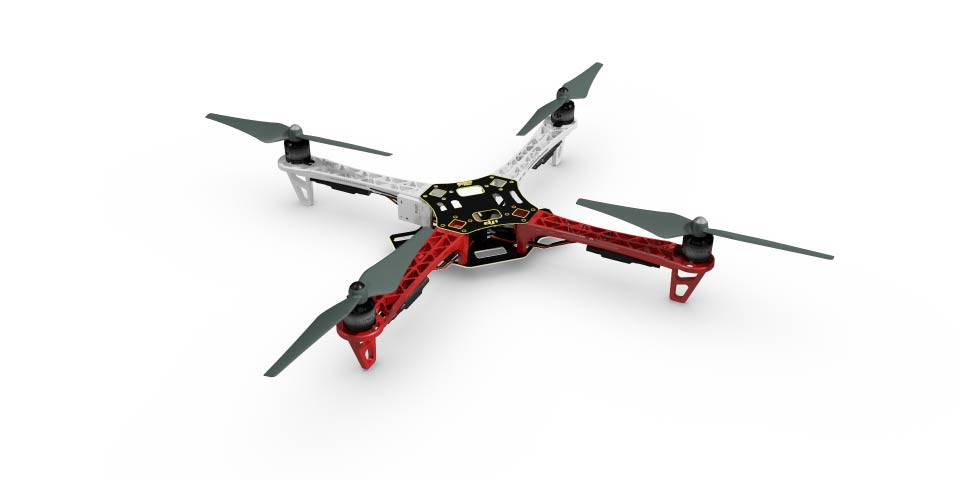
\includegraphics[width=0.9\textwidth] {images/hardware/f450.jpg} 
	\caption{DJI F450 Flamewheel Kit}
	\label{fig:f450}
\end{figure}


\subsection{Flight-Controller}

Der Flight-Controller ist das Herzstück eines Quadcopters. Im Unterschied zu anderen Ferngesteuerten Fahr- und Flugzeugen kann ein Multicopter nur über ein Fly-by-Wire System kontrolliert werden. Das heisst alle Befehle, die von der Fernbedienung kommen, müssen interpretiert und umgewandelt werden, damit die Motoren eine Bewegung in die gewünschte Richtung zu erzeugen können. In Kombination mit einem GPS Modul (Abb. \ref{fig:gps-module}) ermöglich der Controller verschiedene Flugmodi, wie beispielsweise das Schweben an einem Punkt oder automatisches abfliegen von Wegpunkten.

Als Flight-Controller setzen wir ein Pixhawk ein. Es ist sehr vielseitig und kann gut mit zusätzlichen Sensoren erweitert werden, ausserdem unterstützt es gängige Firmwares, die auch auf günstigeren Controllern laufen. Als Firmware für das Pixhawk setzen wir ArduCopter ein, da sie komplett Open-Source ist und auch bei vielen anderen Projekten eingesetzt wird. Sie unterstützt ausserdem das MAV-Link Protokoll, das es ermöglicht verschiedene Hardware über den USB Port anzusprechen.

\begin{figure}[h]
	\centering
	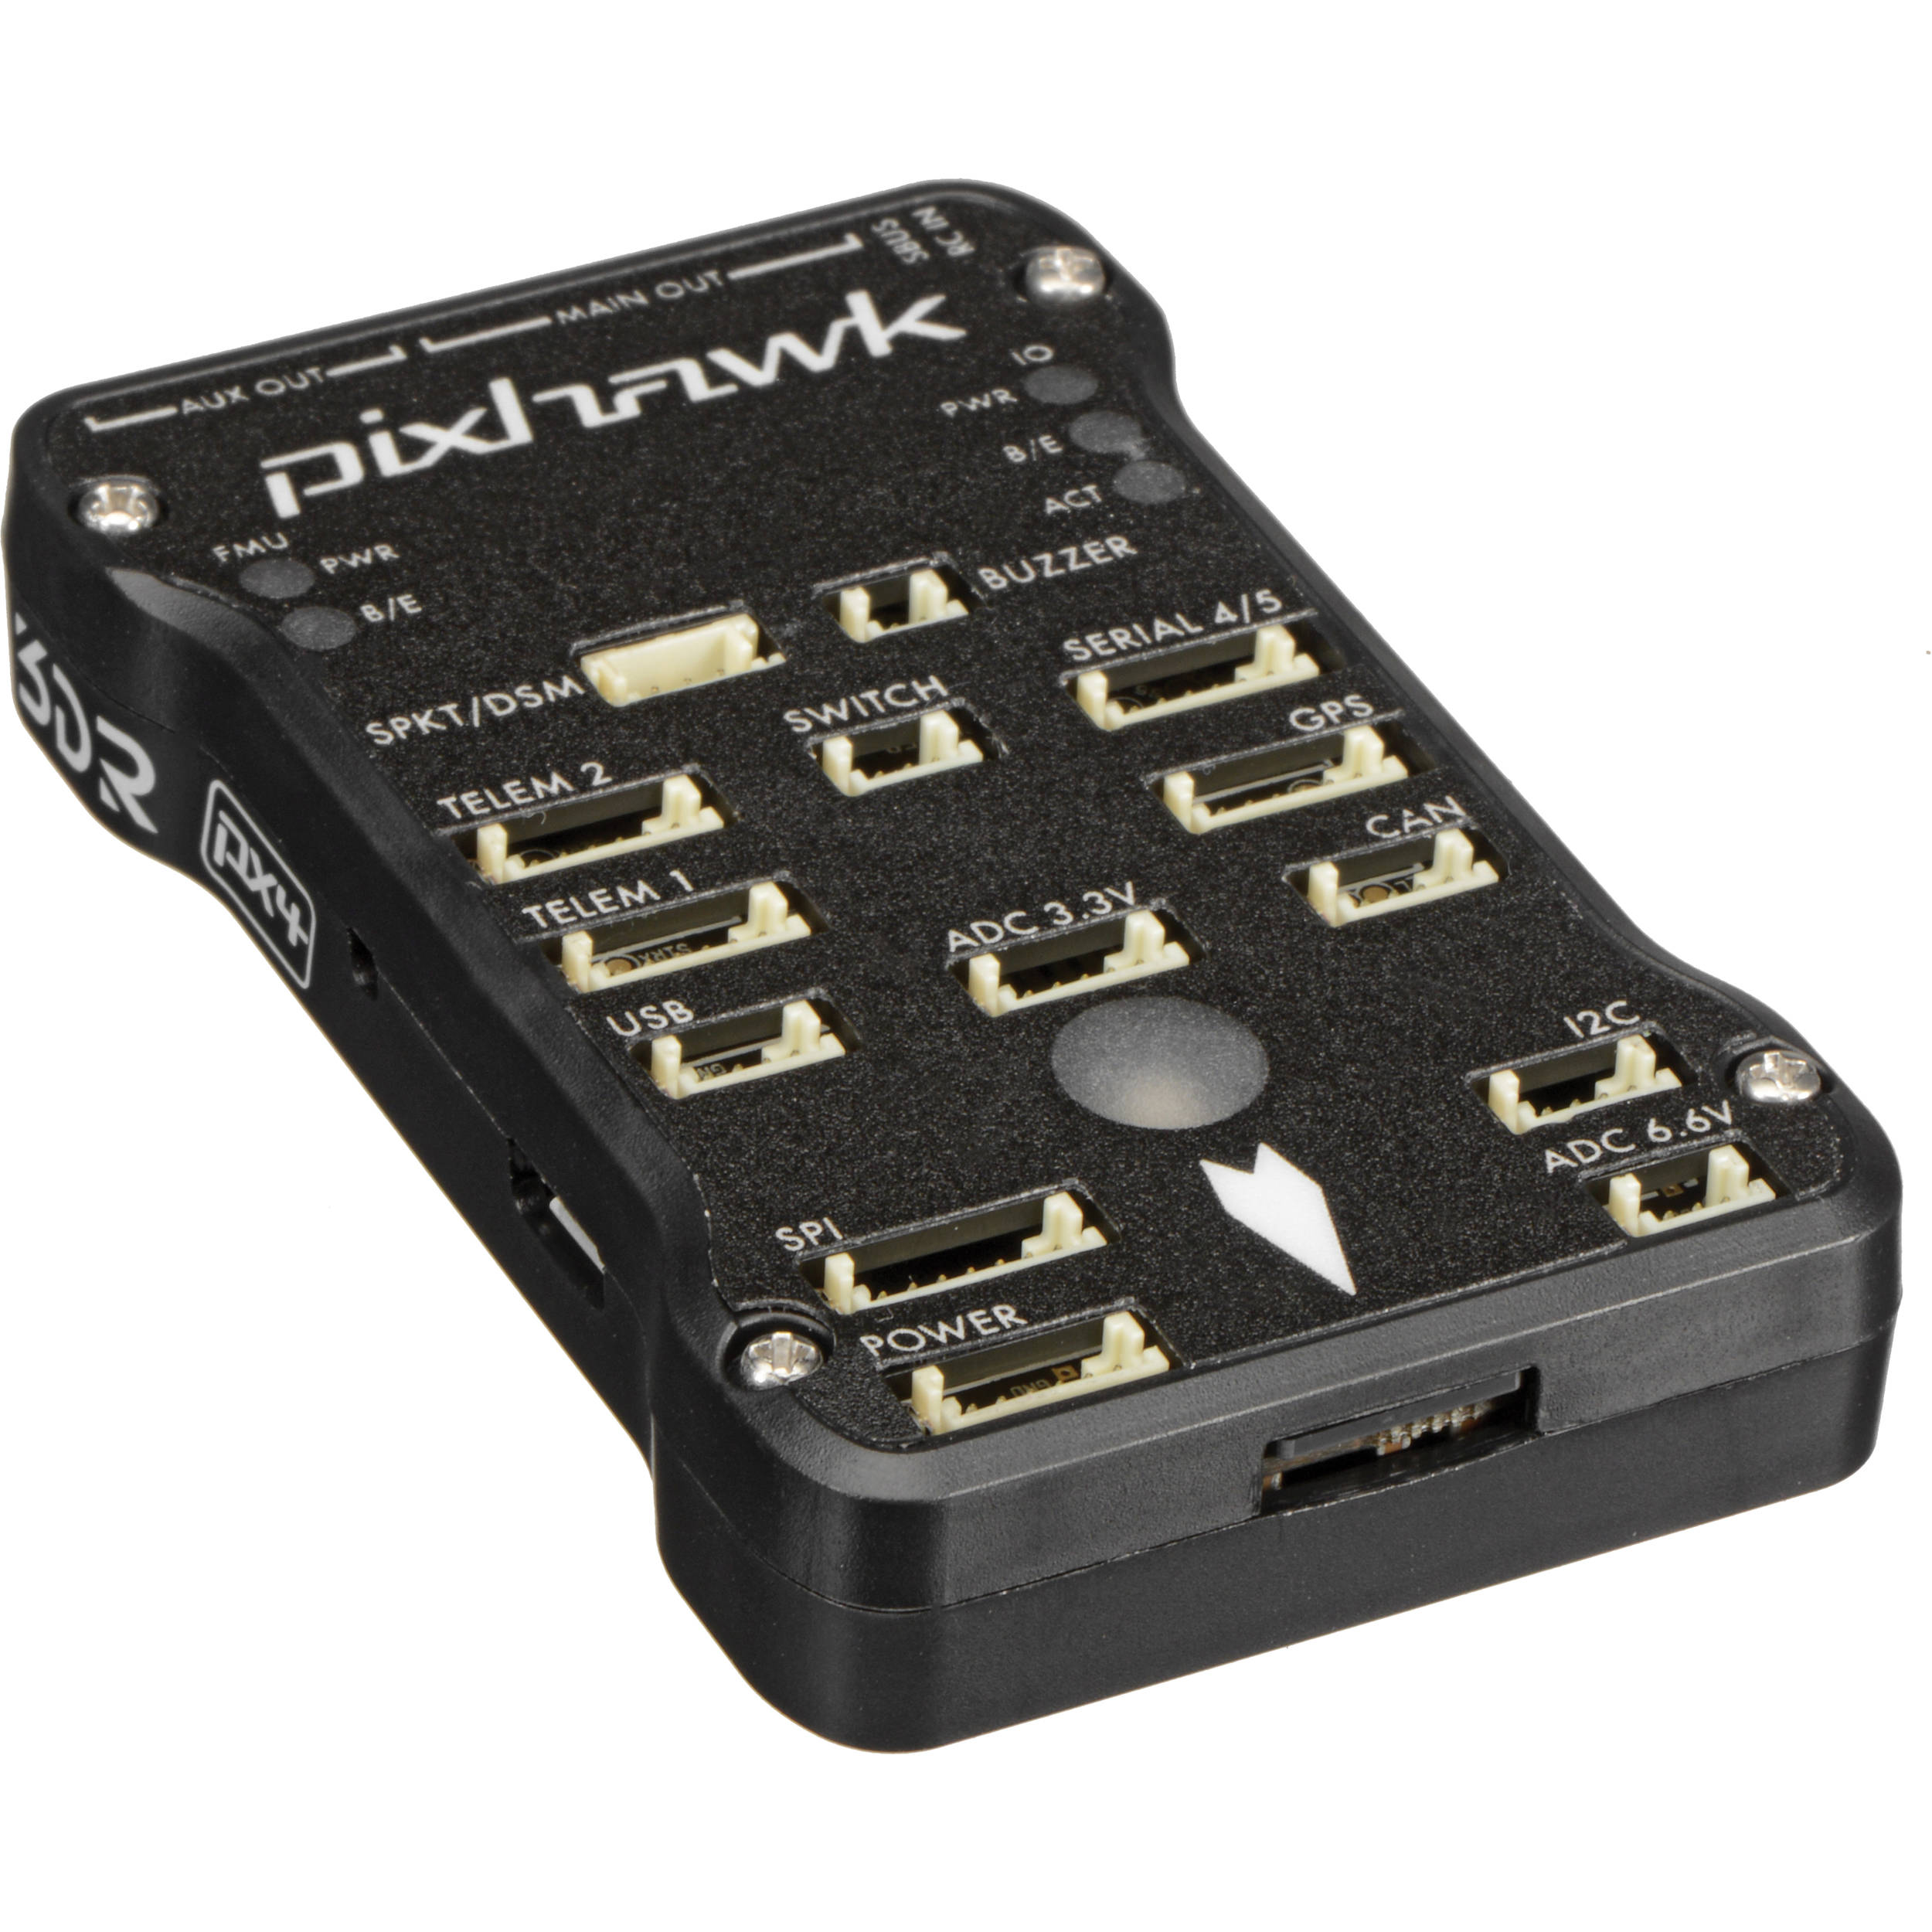
\includegraphics[width=0.3\textwidth] {images/hardware/pixhawk.jpg} 
	\caption{Pixhawk Flight-Controller}
	\label{fig:pixhawk}
\end{figure}

\begin{figure}[h]
	\centering
	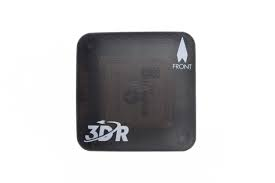
\includegraphics[width=0.3\textwidth] {images/hardware/gps-module.jpg} 
	\caption{GPS-Modul für Pixhawk}
	\label{fig:gps-module}
\end{figure}

\subsection{Ausbaustufen}

Während des Projekts wurden die Hardware laufend den Bedürfnissen angepasst. Daher gibt es mehrere Prototypen, die für die Versuche genutzt wurden.

\subsubsection{Prototyp 1}

Um das Zusammenspiel der Hardwarekomponenten zu testen und erste Versuche mit dem GPS und den verschiedenen Flugmodi zu sammeln, wurde sehr schnell ein Prototyp gebaut.

\begin{figure}[h]
	\centering
	\includegraphics[width=0.9\textwidth] {images/hardware/prototype1.jpg} 
	\caption{Erster Prototyp ohne Landegestellt und ohne Smartphone}
	\label{fig:prototyp-1}
\end{figure}

\subsection{Tests}

Um die Anwendungsmöglichkeiten eines solchen Multicopters auszuloten wurden diverse Experimente durchgeführt um die Leistungsfähigkeit und die Einschränkungen zu testen. 

\subsubsection{Akku Laufzeittest}
Um die maximale Akku Laufzeit zu testen wurde die Drohne ohne zusätzliches Gewicht gestartet, etwa 1.5m über dem Boden schweben gelasswen und die Zeit gemessen. Dabei versucht die Drohne die Postion zu halten, bei Abweichung wurde aktiv korrigiert. \\

\begin{tabularx}{\textwidth}{|c|c|c}
    \hline
    \textbf{Akku} & \textbf{Gewicht}  & \textbf{Laufzeit} \\
    3S & Handy 150g & 16min 29s \\

\end{tabularx}\\

\subsubsection{Tragfähigkeitstests}

Um das maximale Gewicht zu prüfen, das bei einer Präsentation auf unsere Drohnen geladen werden kann, wurden Tests mit dem Zielgewicht von ca. 500g gemacht.Dies Entspricht dem Gewicht einer PET-Flasche eines beliebigen Getränkeherstellers. Ausserdem war auch das Mobiltelefon (ca. 150g) auch auf der Drohne angebracht.  \\

\begin{tabularx}{\textwidth}{|c|c|c|c|X|}
	\hline
	\textbf{Nutzlast} & \textbf{Akku Typ} & \textbf{Nötige Leistung }& \textbf{Erwartete Flugzeit } & \textbf{Subjektives Flugverhalten }\\
	\hline \hline
	500g & 3S & ca. 75\%  & n.A. & Ziemlich Träge, mehr Gewicht wäre kritisch\\
	\hline
	500g & 4S & ca. 45\%  & n.A. & Gewicht kaum Spürbar\\
	\hline  
\end{tabularx}\\

Auch mit 3S Akkus scheint es also möglich eine PET-Flasche zu transportieren. 

\section{Libraries}

\subsection{Server}


\subsection{Onboard App}
\begin{tabularx}{\textwidth}{|X|X|c|X|}
	\hline
	\textbf{Name} & \textbf{Verwendungszweck} & \textbf{Version} & \textbf{Lizenz} \\
	\hline \hline
	DroneKit-Android Client library & Android API für MAV-Link Protokoll (Ansteuerung der Drohne) & 1.5.1 & Apache 2.0\\
	\hline 
	AMQP Messaging Library & Messaging für Android & 3.6.0 &  Mozilla Public License 1.1, GPL 2,  Apache 2.0 \\
	\hline 
	Lyra  & High availability Messaging & 0.4.3 &  Apache 2.0 \\
	\hline 
\end{tabularx}
\subsection{User App}


